\documentclass[conference]{IEEEtran}
\usepackage[utf8]{inputenc}
\usepackage[spanish,es-nodecimaldot]{babel}
\usepackage{graphicx}
\usepackage{amsmath}
\usepackage{booktabs}
\usepackage{cite}
\usepackage{hyperref}
\usepackage{float}

\graphicspath{{../../outputs/figures/}}

\title{Clasificación de Tumores Cerebrales en MRI mediante
Redes Neuronales Convolucionales propias sobre el Dataset
\textit{Brain Tumor Classification MRI}}

\author{\IEEEauthorblockN{Abel Albuez Sánchez, Daniel Rios,
Juan Torres y Javier Esquivel}
\IEEEauthorblockA{Maestría en Analítica para Inteligencia de
Negocios (MAIN)\\
Pontificia Universidad Javeriana, Bogotá D.C., Colombia\\
Profesor: Julio Omar Palacio Niño, M.Sc. \quad
Aprendizaje Profundo \quad 2026}}

\begin{document}
\maketitle

\begin{abstract}
La clasificación automática de tumores cerebrales en imágenes
de resonancia magnética (MRI) es una tarea relevante de apoyo
al diagnóstico radiológico. Este trabajo aborda la clasificación
de cuatro categorías ---\textit{glioma}, \textit{meningioma},
\textit{pituitary} y \textit{no\_tumor}--- sobre el dataset
público \textit{Brain Tumor Classification MRI} de Kaggle
($3\,264$ imágenes), comparando tres arquitecturas
convolucionales \emph{propias} entrenadas desde cero, sin
\textit{transfer learning}. Las redes evaluadas son una
CNN \textit{baseline} de 3 capas convolucionales, una CNN
profunda de 10 capas con \textit{Batch Normalization} y
\textit{Dropout2d}, y MRIResNet, una arquitectura residual con
atención \textit{Squeeze-and-Excitation} y preprocesamiento
multimodal CLAHE+Sobel de 5 canales. MRIResNet alcanza el
mejor F1-macro sobre el \textit{holdout} oficial ($0{,}6593$),
$+3{,}41$ pp sobre el \textit{baseline}, mientras que la CNN
profunda confirma que \textit{Batch Normalization} requiere un
régimen de hiperparámetros propio para no colapsar. Una caída
sistemática de $\sim 30$ puntos entre validación y prueba
indica un \textit{distribution shift} entre las particiones
oficiales que ningún aumento de capacidad resuelve por completo.
\end{abstract}

\begin{IEEEkeywords}
redes neuronales convolucionales, clasificación de imágenes,
tumores cerebrales, MRI, aprendizaje profundo, F1-Score macro
\end{IEEEkeywords}

\section{Introducción}

El diagnóstico temprano de tumores cerebrales constituye uno de
los retos más relevantes de la neuro-oncología contemporánea.
La resonancia magnética (MRI, \textit{Magnetic Resonance
Imaging}) es la modalidad de imagen de referencia para la
detección y caracterización de estas lesiones; sin embargo, su
interpretación depende fuertemente de la experiencia del
radiólogo y está sujeta a variabilidad inter-observador. En
este contexto, los sistemas de apoyo basados en aprendizaje
profundo han mostrado resultados prometedores como
herramientas de cribado y segunda opinión, capaces de procesar
grandes volúmenes de estudios de forma consistente.

Este trabajo propone, entrena y evalúa tres arquitecturas
convolucionales \emph{propias} sobre el dataset público
\textit{Brain Tumor Classification MRI}~\cite{sartaj2020dataset}.
A diferencia de la literatura mayoritaria sobre el corpus, que
emplea \textit{fine-tuning} de redes pre-entrenadas
(VGG16~\cite{simonyan2014very}, ResNet50~\cite{he2016resnet},
MobileNetV2), las tres redes se entrenan desde cero. El énfasis
metodológico se sitúa, por tanto, en la comprensión del impacto
de cada bloque arquitectónico ---\textit{Batch Normalization},
\textit{Dropout2d}, conexiones residuales, atención de canales,
preprocesamiento estructural--- sobre el rendimiento y la
generalización a una partición de prueba afectada por
\textit{distribution shift}.

\textbf{Contribuciones.} (i)~Replicación crítica de OkanNet,
mostrando que la incorporación de \textit{Batch Normalization}
bajo el régimen de hiperparámetros del \textit{baseline} (lr
$=10^{-3}$, batch~$=32$) degrada el F1-macro en $20{,}19$ pp,
y demostrando que una CNN profunda con BN entrenada bajo un
régimen propio (lr~$=5{\times}10^{-4}$, batch~$=64$, AdamW)
recupera ese rendimiento. (ii)~Diseño de MRIResNet, una
arquitectura residual con atención SE que incorpora un
preprocesamiento multimodal explícito (CLAHE + Sobel) y supera
al \textit{baseline} usando $\sim 4{\times}$ menos parámetros.
(iii)~Análisis del \textit{distribution shift} entre las
particiones oficiales \textit{Training}/\textit{Testing} del
dataset, identificándolo como la limitación dominante de
generalización por encima de la capacidad arquitectónica.

\section{Objetivos}

\textbf{Objetivo general.} Diseñar, entrenar y evaluar tres
arquitecturas propias de redes neuronales convolucionales para
la clasificación automática de imágenes MRI cerebrales en cuatro
categorías (\textit{glioma}, \textit{meningioma},
\textit{no\_tumor} y \textit{pituitary}), sin emplear pesos
preentrenados.

\textbf{Objetivos específicos.}
(i)~Construir un \textit{baseline} convolucional ligero (Modelo~1)
que sirva como referencia y replicar OkanNet~\cite{okannet2026}
como contraste académico del impacto de BN bajo un régimen de
hiperparámetros idéntico.
(ii)~Diseñar una CNN profunda (Modelo~2) con BN y
\textit{Dropout2d} en cada bloque, junto a una variante con
\textit{Global Average Pooling} (GAP), para aislar el aporte
del cabezal denso.
(iii)~Construir un Modelo~3 más avanzado (MRIResNet)
con bloques residuales, atención SE y preprocesamiento
multimodal CLAHE+Sobel desde cero.
(iv)~Reportar y comparar las cuatro métricas estándar
(\textit{Accuracy}, \textit{Precision}, \textit{Recall},
F1-Score \textit{macro-averaged}) y las matrices de confusión
sobre el \textit{holdout} oficial.

\section{Análisis del Problema}

\subsection{Dataset}
El dataset \textit{Brain Tumor Classification MRI}
contiene $3\,264$ imágenes de resonancia cerebral en cuatro
clases. La partición oficial entrega $2\,870$ imágenes para
entrenamiento y $394$ para prueba
(Tabla~\ref{tab:art-dist}).

\begin{table}[!t]
\centering
\caption{Distribución de imágenes por clase y partición.}
\label{tab:art-dist}
\footnotesize
\begin{tabular}{lrrr}
\toprule
\textbf{Clase} & \textbf{Train} & \textbf{Test} & \textbf{Total} \\
\midrule
\texttt{glioma\_tumor}     & 826 & 100 & 926 \\
\texttt{meningioma\_tumor} & 822 & 115 & 937 \\
\texttt{no\_tumor}         & 395 & 105 & 500 \\
\texttt{pituitary\_tumor}  & 827 &  74 & 901 \\
\midrule
\textbf{Total}             & $\mathbf{2\,870}$ & $\mathbf{394}$ & $\mathbf{3\,264}$ \\
\bottomrule
\end{tabular}
\end{table}

\subsection{Desafíos identificados}

\textbf{Desbalance de clases.} \textit{no\_tumor} es la clase
minoritaria ($\sim$1:2 respecto a las clases tumorales). Para
mitigarlo se incorpora \textit{class\_weight} balanceado en la
función de pérdida \texttt{CrossEntropyLoss}.

\textbf{Heterogeneidad dimensional.} Las imágenes presentan
resoluciones entre $59{\times}80$\,px y $1024{\times}768$\,px.
Se redimensiona todo a $224{\times}224$\,px, un compromiso
entre detalle anatómico y costo computacional consistente con
las arquitecturas CNN modernas.

\textbf{Variabilidad fotométrica.} Los \textit{gliomas} son
hipointensos (media $36{,}23$, mediana $14$), los
\textit{pituitarios} más concentrados (mediana $50$) y
\textit{no\_tumor} presenta la mayor desviación estándar
($59{,}63$), reflejando la diversidad anatómica del cerebro
sano. Estas diferencias constituyen señales explotables por la
CNN a nivel de filtros convolucionales.

\textbf{Distribution shift.} Como se documenta en
Resultados, los tres modelos sufren una caída sistemática de
$\sim 30$ puntos entre F1-macro de validación
y de prueba, atribuible a la divergencia distribucional entre
las particiones oficiales del corpus.

\subsection{Métricas y protocolo}

Se reportan \textit{Accuracy}, \textit{Precision},
\textit{Recall} y F1-Score, todas en su variante
\textit{macro-averaged} dado el desbalance del corpus, junto a
la matriz de confusión normalizada por clase real. El F1-macro
es la métrica principal de comparación. Sobre \textit{Training}
se aplica una división interna 80/20 para validación; el
conjunto \textit{Testing} se reserva como \textit{holdout}
independiente y se usa únicamente para la evaluación final
reportada en la Sección~\ref{sec:art-resultados}.

\section{Construcción, Entrenamiento e Implementación}

\subsection{Modelo 1 --- CNN Baseline y OkanNet}
\label{sec:art-m1}

El Modelo~1 implementa una CNN \textit{baseline} ligera
inspirada en OkanNet~\cite{okannet2026} y en la red de
Gupta~\textit{et al.}~\cite{gupta2023}: tres bloques
secuenciales \texttt{Conv2D}$(3{\times}3)$--\texttt{ReLU}--%
\texttt{MaxPool2D}$(2{\times}2)$ con filtros $16{\to}32{\to}64$,
seguidos de un cabezal denso \texttt{Linear}$(50\,176{\to}128)$%
--\texttt{ReLU}--\texttt{Dropout}$(0{,}5)$--\texttt{Linear}$(128{\to}4)$.
La inicialización es \textit{Kaiming Normal}
(\texttt{fan\_out} para \texttt{Conv2D}, \texttt{fan\_in} para
\texttt{Linear}). Total: $6\,446\,756$ parámetros, dominados al
$99{,}6$\,\% por la primera capa totalmente conectada.

Como contraste académico se replica \textbf{OkanNet}, idéntica
al \textit{baseline} pero con \texttt{BatchNorm2D} tras cada
\texttt{Conv2D} ($+224$ parámetros). Los hiperparámetros de
entrenamiento se mantienen idénticos entre ambas redes para
aislar el efecto de BN.

\textbf{Hiperparámetros (M1).} Adam ($\beta_1{=}0{,}9$,
$\beta_2{=}0{,}999$), lr$_0{=}10^{-3}$,
\texttt{ReduceLROnPlateau}(factor $0{,}5$, paciencia $3$),
\texttt{CrossEntropyLoss} con \texttt{class\_weight}, batch
$=32$, $40$ épocas máx., \textit{early stopping} con paciencia
$7$ sobre F1-macro de validación, \textit{seed} $42$.

\subsection{Modelo 2 --- CNN Profunda con BN y Dropout}
\label{sec:art-m2}

El Modelo~2 se motiva en el colapso de OkanNet bajo el régimen
del Modelo~1: la hipótesis es que el fallo no se debe a BN como
técnica sino a su sensibilidad al \textit{learning rate}
y al tamaño de \textit{batch}. El Modelo~2 contrasta esta
hipótesis con una red sustancialmente más profunda
---$10$ capas convolucionales VGG-style frente a $3$ del
baseline--- entrenada con un régimen propio: AdamW,
lr=$5{\times}10^{-4}$, batch=$64$, weight decay=$10^{-4}$,
$50$ épocas máx.

Se construyen dos variantes que comparten el mismo
\textit{backbone} convolucional pero difieren en el cabezal:

\begin{itemize}
  \item \textbf{DeepCNN-BN.} Cabezal denso clásico con
        \texttt{AdaptiveAvgPool2D}$(2,2) \to$
        \texttt{Linear}$(2048{\to}256) \to$ BN1D $\to$ ReLU $\to$
        \texttt{Dropout}$(0{,}5) \to$ \texttt{Linear}$(256{\to}4)$.
        Total: $5\,240\,292$ parámetros.
  \item \textbf{DeepCNN-BN-GAP.} \textit{Global Average
        Pooling} en lugar del FC denso:
        \texttt{AdaptiveAvgPool2D}$(1,1) \to$
        \texttt{Dropout}$(0{,}5) \to$ \texttt{Linear}$(512{\to}4)$.
        Total: $4\,716\,260$ parámetros ($-524$\,K respecto a
        la variante FC).
\end{itemize}

El \textit{backbone} se compone de cinco bloques con dos
\texttt{Conv2D}$(3{\times}3)$ + \texttt{BatchNorm2D} + ReLU
cada uno, \texttt{MaxPool}$(2{\times}2)$ y \texttt{Dropout2D}
de tasa creciente ($0{,}10 \to 0{,}30$) entre bloques. La
progresión de filtros es $32{\to}64{\to}128{\to}256{\to}512$.
El último bloque omite el \texttt{MaxPool} para producir
salida $14{\times}14$, requisito de divisibilidad del backend
MPS bajo \texttt{AdaptiveAvgPool2D}.

\subsection{Modelo 3 --- MRIResNet con Atención SE}
\label{sec:art-m3}

El Modelo~3 (\textbf{MRIResNet}) extiende el \textit{baseline}
en tres ejes complementarios.

\textbf{(a)~Preprocesamiento multimodal de 5 canales.} En lugar
de RGB $(B,3,224,224)$, el modelo recibe un tensor
$(B,5,224,224)$ generado mediante
CLAHE~\cite{zuiderveld1994clahe}
(\textit{clipLimit}~$=2{,}0$, \textit{tileGrid}~$=8{\times}8$)
sobre la imagen en escala de grises ---que mejora el contraste
local sin amplificar ruido global--- seguido de filtro Sobel
$G{=}\sqrt{G_x^2{+}G_y^2}$ sobre la imagen CLAHE para extraer
gradientes espaciales. Los canales finales son
$[R,G,B,\text{CLAHE},\text{Sobel}]$, normalizados canal a canal
con estadísticos de \textit{Training}. Este diseño está
conceptualmente inspirado en los hallazgos de Hubel y
Wiesel~\cite{hubel1959receptive} sobre selectividad
orientacional en la corteza visual primaria.

\textbf{(b)~Bloques residuales.} Cada bloque aprende
$\mathcal{F}(\mathbf{x}){+}\mathbf{x}$~\cite{he2016resnet}
con estructura interna
\texttt{Conv}$(3{\times}3)$-BN-ReLU-\texttt{Conv}$(3{\times}3)$-BN%
$\oplus\mathbf{x}$-ReLU. Cuando los canales de entrada y salida
difieren, el camino \textit{skip} incorpora una proyección
\texttt{Conv}$(1{\times}1)$+BN.

\textbf{(c)~Atención Squeeze-and-Excitation
(SE)~\cite{hu2018senet}.} El módulo SE recalibra los canales
en tres etapas: \emph{squeeze} mediante GAP global, \emph{excitation}
mediante \texttt{FC}--ReLU--\texttt{FC}--Sigmoid con ratio de
reducción $r{=}8$, y reescalado multiplicativo
$\hat{x}_c{=}s_c\cdot x_c$.

La arquitectura final consta de $1\,676\,284$ parámetros
entrenables (apenas el $26$\,\% del \textit{baseline}), gracias
al uso de \textit{Global Average Pooling} en el cabezal. Se
entrena con AdamW (lr~$=10^{-4}$, \textit{weight decay}~$=10^{-4}$),
batch~$=32$, $50$ épocas máx., \textit{early stopping} con
paciencia~$10$ sobre F1-macro de validación.

\subsection{Implementación}

Toda la implementación se realiza en Python con PyTorch sobre
Apple Silicon (backend MPS). El código se organiza en
\texttt{models/model\{1,2,3\}/} como tres paquetes
auto-contenidos, con utilidades compartidas en
\texttt{models/common/}. Cada modelo expone una CLI
(\texttt{train.py --arch <name>}) y reportes incrementales por
época en CSV.

\section{Resultados}
\label{sec:art-resultados}

\subsection{Métricas globales sobre Testing}

La Tabla~\ref{tab:art-metricas-global} reporta las métricas
sobre el \textit{holdout} oficial de $394$ imágenes.

\begin{table}[!t]
\centering
\caption{Métricas globales sobre \textit{Testing}.}
\label{tab:art-metricas-global}
\renewcommand{\arraystretch}{1.15}
\footnotesize
\begin{tabular}{@{}lcccc@{}}
\toprule
\textbf{Modelo} & \textbf{Acc.} & \textbf{Prec.} &
\textbf{Rec.} & \textbf{F1-Macro} \\
\midrule
Baseline (M1)         & $0{,}6751$ & $0{,}7443$ & $0{,}6508$ & $0{,}6252$ \\
OkanNet (comp.)       & $0{,}4467$ & $0{,}4901$ & $0{,}4634$ & $0{,}4233$ \\
DeepCNN-BN (M2)       & $0{,}6472$ & $0{,}7403$ & $0{,}6351$ & $0{,}5961$ \\
DeepCNN-BN-GAP (M2)   & $0{,}5558$ & $0{,}6765$ & $0{,}5482$ & $0{,}5176$ \\
MRIResNet (M3)        & $\mathbf{0{,}7107}$ & $\mathbf{0{,}7947}$ & $\mathbf{0{,}6992}$ & $\mathbf{0{,}6593}$ \\
\bottomrule
\end{tabular}
\end{table}

\begin{table}[!t]
\centering
\caption{F1-Score por clase sobre \textit{Testing}.}
\label{tab:art-f1-clase}
\renewcommand{\arraystretch}{1.15}
\footnotesize
\setlength{\tabcolsep}{3pt}
\begin{tabular}{@{}lccccc@{}}
\toprule
\textbf{Clase} & \textbf{Base.} & \textbf{Okan.} &
\textbf{DeepCNN} & \textbf{GAP} & \textbf{MRIResNet} \\
\midrule
glioma     & $\mathbf{0{,}3307}$ & $0{,}2597$ & $0{,}2759$ & $0{,}2735$ & $0{,}2906$ \\
mening.    & $0{,}7766$ & $0{,}2517$ & $0{,}7137$ & $0{,}5676$ & $\mathbf{0{,}7912}$ \\
no\_tumor  & $0{,}7445$ & $0{,}5337$ & $0{,}7331$ & $0{,}6355$ & $\mathbf{0{,}7816}$ \\
pituitary  & $0{,}6491$ & $0{,}6479$ & $0{,}6618$ & $0{,}5938$ & $\mathbf{0{,}7737}$ \\
\bottomrule
\end{tabular}
\end{table}

\subsection{Modelo 1 (Baseline + OkanNet)}

El \textit{baseline} alcanza F1-macro de $0{,}6252$. La
incorporación de BN sin ajuste de hiperparámetros (OkanNet) lo
desploma a $0{,}4233$ ($-20{,}19$ pp), con convergencia
inestable y disparo de \textit{early stopping} en la
época~$17$. Este resultado no invalida BN como técnica, sino
que evidencia su sensibilidad al régimen
lr~$=10^{-3}$/batch~$=32$. El sesgo
\textit{glioma}$\to$\textit{meningioma} domina los errores: el
$79$\,\% de los gliomas reales se asigna mayoritariamente como
meningioma, generando Precision alta ($0{,}7778$) pero Recall
bajísimo ($0{,}2100$) sobre la clase \textit{glioma}.

\subsection{Modelo 2 (DeepCNN-BN y DeepCNN-BN-GAP)}

DeepCNN-BN alcanza $0{,}5961$ de F1-macro
($+17{,}28$ pp sobre OkanNet, $-2{,}91$ pp sobre el
\textit{baseline}). Las curvas de validación son
monótonas crecientes hasta $0{,}9112$ en la época~$50$, sin
disparar \textit{early stopping}, lo que confirma que BN
funciona bajo el régimen adaptado (AdamW
lr~$=5{\times}10^{-4}$, batch~$=64$, \textit{weight
decay}~$=10^{-4}$).

La variante GAP rinde $7{,}85$ pp por debajo del FC denso
($0{,}5176$ vs $0{,}5961$), pese a compartir el
\textit{backbone}: los $\sim 524$\,K parámetros adicionales
del cabezal FC sí aportan capacidad discriminativa real en
este corpus, particularmente en \textit{meningioma}
($+14{,}6$ pp) y \textit{no\_tumor} ($+9{,}8$ pp). La hipótesis
``GAP rinde equivalentemente cuando el \textit{backbone} es
suficientemente profundo'' no se sostiene aquí.

\begin{figure}[!t]
\centering
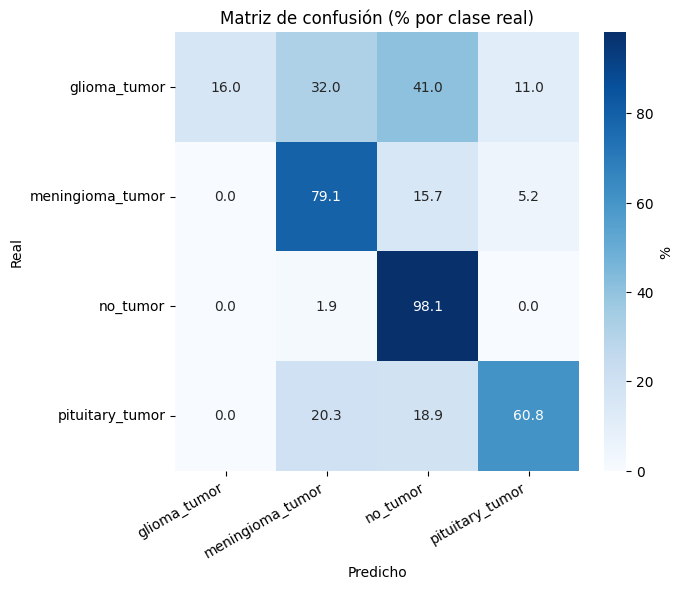
\includegraphics[width=\linewidth]{model-2/confusion_deep.png}
\caption{Matriz de confusión normalizada de DeepCNN-BN sobre
\textit{Testing}.}
\label{fig:art-cm-deep}
\end{figure}

\begin{figure}[!t]
\centering
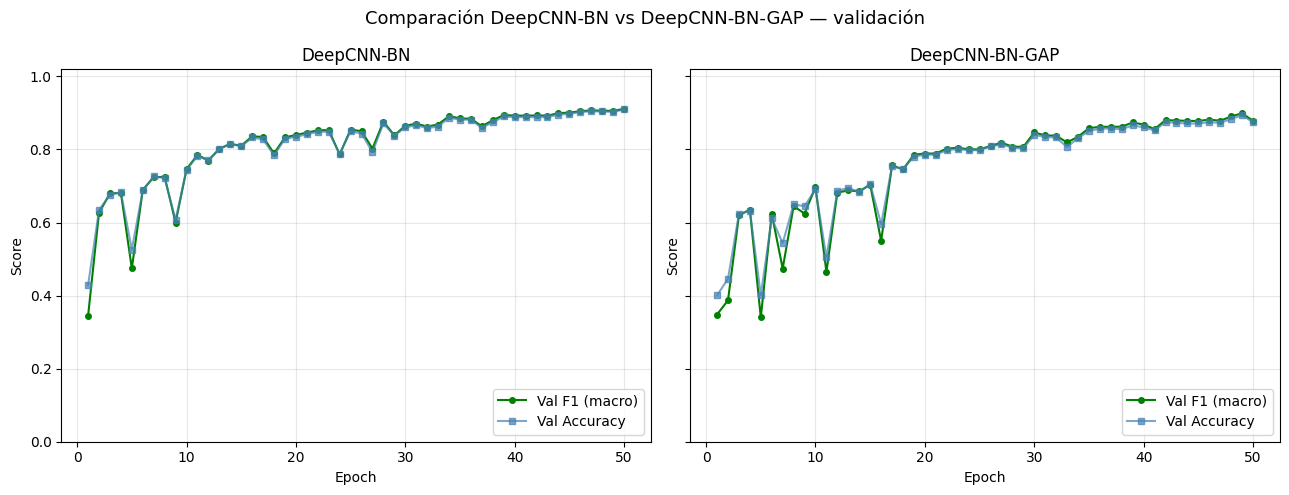
\includegraphics[width=\linewidth]{model-2/comparacion_deep_vs_deepgap.png}
\caption{F1-macro de validación de DeepCNN-BN y
DeepCNN-BN-GAP a lo largo del entrenamiento. Ambas convergen
sin disparar \textit{early stopping}, contrastando con la
inestabilidad de OkanNet.}
\label{fig:art-comp-m2}
\end{figure}

\subsection{Modelo 3 (MRIResNet)}

MRIResNet alcanza el mejor F1-macro del trabajo
($\mathbf{0{,}6593}$), $+3{,}41$ pp sobre el \textit{baseline}
y $+6{,}32$ pp sobre DeepCNN-BN, usando $\sim 4{\times}$ menos
parámetros que el \textit{baseline}. La mejora se concentra en
las tres clases ``aprendibles'': \textit{meningioma}~$+1{,}46$ pp,
\textit{no\_tumor}~$+3{,}71$ pp y, especialmente,
\textit{pituitary}~$+12{,}46$ pp respecto al \textit{baseline}.
La clase \textit{glioma\_tumor} sigue siendo el cuello de
botella en los tres modelos (F1 entre $0{,}26$ y $0{,}33$),
consistente con una hipótesis de divergencia distribucional:
los gliomas del \textit{Testing} parecen provenir de subtipos
o protocolos sub-representados en \textit{Training}, lo cual
no se compensa con mayor capacidad arquitectónica.

\begin{figure}[!t]
\centering
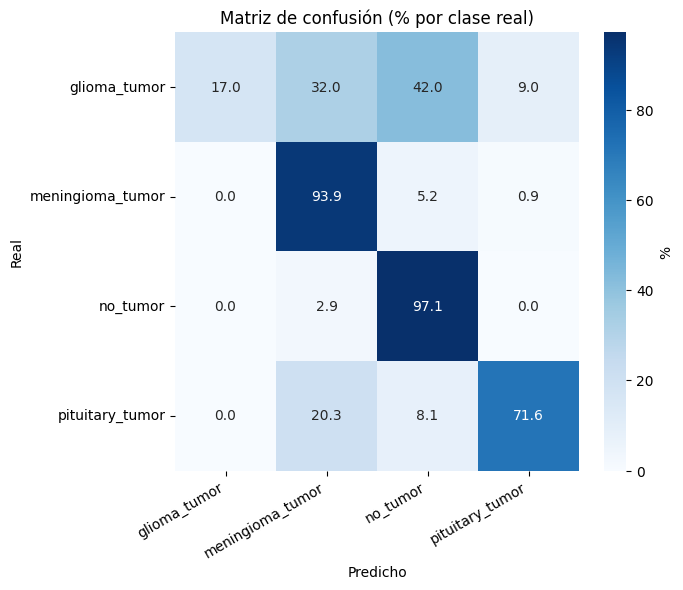
\includegraphics[width=\linewidth]{model-3/confusion_mriresnet.png}
\caption{Matriz de confusión normalizada de MRIResNet sobre
\textit{Testing}.}
\label{fig:art-cm-m3}
\end{figure}

\subsection{Distribution shift}

Los cinco modelos exhiben una caída sistemática de
$\sim 30$~pp entre F1-macro de validación y de prueba
(\textit{baseline}: $0{,}92 {\to} 0{,}63$;
DeepCNN-BN: $0{,}91{\to}0{,}60$;
MRIResNet: $\sim 0{,}90{\to}0{,}66$). Pese a triplicar la
profundidad, añadir BN, regularización con \textit{weight
decay} y preprocesamiento multimodal, el F1-macro de prueba
mejora solo $3{,}41$ pp respecto al \textit{baseline}. Esto
indica que el factor dominante de generalización en este corpus
\textbf{no es la capacidad del modelo sino el
\textit{distribution shift}} entre las particiones oficiales.

\section{Conclusiones}

Las CNN propias entrenadas desde cero alcanzan un F1-macro de
hasta $0{,}6593$ sobre el \textit{holdout} oficial, valor que
sitúa al sistema como herramienta de \emph{cribado}
complementaria al criterio radiológico, pero \emph{no} como
clasificador clínico autónomo. La clase \textit{glioma\_tumor}
es el cuello de botella sistemático en los tres modelos, con
F1 entre $0{,}26$ y $0{,}33$ y Recall por debajo del $25$\,\%
incluso en MRIResNet.

Del análisis comparativo se desprenden tres lecciones
metodológicas: (i)~\textit{Batch Normalization} no es
intrínsecamente perjudicial; su efectividad depende
críticamente del régimen de entrenamiento, como demuestra el
contraste OkanNet vs DeepCNN-BN. (ii)~Las técnicas avanzadas
(residuales, atención SE, preprocesamiento estructural CLAHE
+ Sobel) aportan ganancias reales pero modestas en
\textit{Testing} ($+3{,}41$ pp en F1-macro), porque la
limitación dominante es distribucional, no arquitectónica.
(iii)~El cabezal denso aporta capacidad discriminativa
relevante frente al GAP en este corpus, contrariamente a la
intuición ``GAP es suficiente si el \textit{backbone} es
profundo''.

\textbf{Limitaciones y trabajo futuro.} La principal limitación
es la pérdida sistemática de $\sim 30$ puntos entre validación
y prueba, atribuible al \textit{split} oficial del dataset y
no a las arquitecturas evaluadas. Las direcciones más
prometedoras son (i)~\textit{transfer learning} desde redes
pre-entrenadas, capaces de capturar invariancias robustas
frente al \textit{shift}, abordado en la fase de
investigación complementaria de este proyecto;
(ii)~\textit{domain adaptation} entre particiones; y
(iii)~validación cruzada estratificada sobre el conjunto
unificado para cuantificar la verdadera capacidad de
generalización de cada modelo independientemente del
\textit{split} oficial.

\begin{thebibliography}{99}
\bibitem{sartaj2020dataset} S.~Bhuvaji, ``Brain Tumor
Classification (MRI),'' Kaggle, 2020.
\bibitem{simonyan2014very} K.~Simonyan and A.~Zisserman, ``Very
deep convolutional networks for large-scale image
recognition,'' \textit{arXiv:1409.1556}, 2014.
\bibitem{he2016resnet} K.~He, X.~Zhang, S.~Ren and J.~Sun,
``Deep residual learning for image recognition,'' in
\textit{CVPR}, 2016.
\bibitem{okannet2026} A.~Uçar and Y.~Kurt, ``OkanNet: a
lightweight CNN for MRI tumor classification,'' 2026.
\bibitem{gupta2023} R.~Gupta \textit{et al.}, ``Classification
of brain tumor images using CNN,'' 2023.
\bibitem{hu2018senet} J.~Hu, L.~Shen and G.~Sun,
``Squeeze-and-excitation networks,'' in \textit{CVPR}, 2018.
\bibitem{hubel1959receptive} D.~H.~Hubel and T.~N.~Wiesel,
``Receptive fields of single neurones in the cat's striate
cortex,'' \textit{J. Physiol.}, vol.~148, 1959.
\bibitem{zuiderveld1994clahe} K.~Zuiderveld, ``Contrast
limited adaptive histogram equalization,'' in \textit{Graphics
Gems IV}, 1994.
\end{thebibliography}

\end{document}
